%%% Template originaly created by Karol Kozioł (mail@karol-koziol.net) and modified for ShareLaTeX use

\documentclass[a4paper,11pt]{article}

\usepackage[T1]{fontenc}
\usepackage[utf8]{inputenc}
\usepackage{graphicx}
\usepackage{xcolor}

\renewcommand\familydefault{\sfdefault}
\usepackage{tgheros}

\usepackage{amsmath,amssymb,amsthm,textcomp}
\usepackage{enumerate}
\usepackage{multicol}
\usepackage{tikz}

\usepackage{geometry}
\geometry{left=25mm,right=25mm,%
bindingoffset=0mm, top=20mm,bottom=20mm}


\linespread{1.3}

\newcommand{\linia}{\rule{\linewidth}{0.5pt}}

% custom theorems if needed
\newtheoremstyle{mytheor}
    {1ex}{1ex}{\normalfont}{0pt}{\scshape}{.}{1ex}
    {{\thmname{#1 }}{\thmnumber{#2}}{\thmnote{ (#3)}}}

\theoremstyle{mytheor}
\newtheorem{defi}{Definition}

% my own titles
\makeatletter
\renewcommand{\maketitle}{
\begin{center}
\vspace{2ex}
{\huge \textsc{\@title}}
\vspace{1ex}
\\
\linia\\
\@author \hfill \@date
\vspace{4ex}
\end{center}
}
\makeatother
%%%

% custom footers and headers
\usepackage{fancyhdr}
\pagestyle{fancy}
\lhead{}
\chead{}
\rhead{}
\lfoot{}
\cfoot{}
\rfoot{Page \thepage}
\renewcommand{\headrulewidth}{0pt}
\renewcommand{\footrulewidth}{0pt}
%

% code listing settings
\usepackage{listings}
\lstset{
    language=lisp,
    basicstyle=\ttfamily\small,
    aboveskip={1.0\baselineskip},
    belowskip={1.0\baselineskip},
    columns=fixed,
    extendedchars=true,
    breaklines=true,
    tabsize=4,
    prebreak=\raisebox{0ex}[0ex][0ex]{\ensuremath{\hookleftarrow}},
    frame=lines,
    showtabs=false,
    showspaces=false,
    showstringspaces=false,
    keywordstyle=\color[rgb]{0.627,0.126,0.941},
    commentstyle=\color[rgb]{0.133,0.545,0.133},
    stringstyle=\color[rgb]{01,0,0},
    numbers=left,
    numberstyle=\small,
    stepnumber=1,
    numbersep=10pt,
    captionpos=t,
    escapeinside={\%*}{*)}
}

%%%----------%%%----------%%%----------%%%----------%%%

\begin{document}
\title{El Despegue - Tarea \textnumero{} 02}

\author{Enrique Giottonini}

\date{OKTOBERFEST}

\maketitle

\section*{Problema 5}
La llamada (bundle ’(”a” ”b” ”c”) 0) es un buen uso de bundle ? ¿qué produce?
¿por qué? \\ \\
Sea $\gamma = (bundle\, s\, n)$ donde $s$ es una lista de caracteres y $n$ el tamaño de los trozos entonces:
\[ (length\,\gamma) = \Big \lceil \dfrac{length(s)}{n}\Big \rceil\]
Por lo que no tiene sentido que $n$ sea igual a 0. En la implementacion de <bundle> esto se refleja en la llamada recursiva estructural.

\begin{lstlisting}[title=bundle]
(define (bundle s n)
  (cond
    [(null? s) null]
    [else
     (cons (implode (take s n))
           (bundle (drop s n) n))]))
\end{lstlisting}

$(drop \,s \,n) = s$ si $n=0$ por lo que la llamada recursiva  en $(bundle\, s\, 0)$ entraria en un loop infinito.
\\
 

\section*{Problema 9}
Dibuja un diagrama como el de la figura anterior($<quicksort>$) pero para la lista ’(11 9 2 18 12
14 4 1) .

\begin{figure}[t]
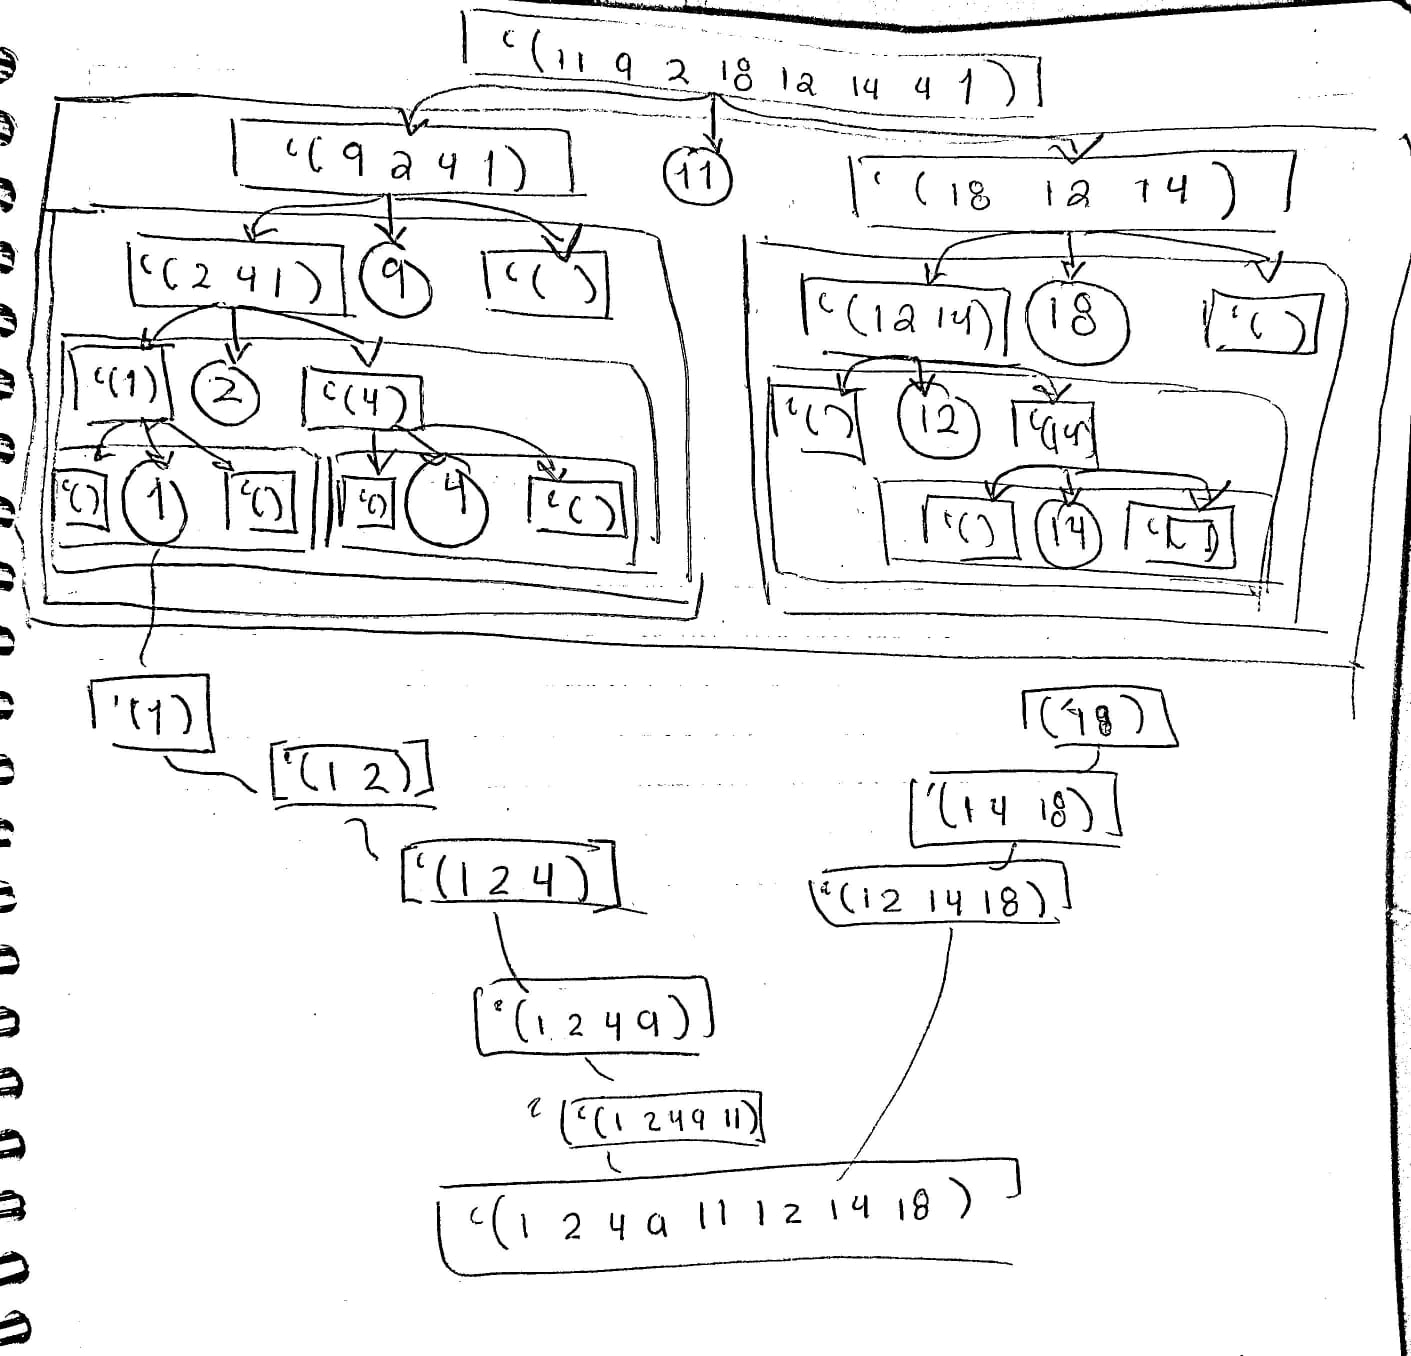
\includegraphics[width=15cm]{img}
\centering
\end{figure}

\newpage
\section*{Problema 11}
Si la entrada a quicksort contiene varias repeticiones de un número, va a regresar
una lista estrictamente más corta que la entrada. Responde el por qué y arregla el problema. \\ \\

La llamada recursiva de quicksort divide el problema (la lista) en 3 partes.
\begin{enumerate}
\item Los que son estrictamente menores al pivote.
\item El elemento
\item Los que son estrictamente mayores al pivote.
\end{enumerate}
\begin{lstlisting}[title=quicksort]
(define (quicksort ls)
  (cond
    [(empty? ls) null]
    [else
     (define pivot (first ls))
     (append (quicksort (smallers ls pivot))
             (list pivot)
             (quicksort (largers ls pivot)))]))
\end{lstlisting}

Una manera de solucionarlo puede ser que en la 2) parte en vez de solo seleccionar el pivote se construya una lista de todas las repeticiones del pivote.
\begin{lstlisting}[title=quicksort]
(define (quicksort ls)
  (cond
    [(empty? ls) null]
    [else
     (define pivot (first ls))
     (append (quicksort (smallers ls pivot))
             (filter (lambda (x) (equal? x pivot)) ls)
             (quicksort (largers ls pivot)))]))
\end{lstlisting}

\section*{Problema 13}
Implementa una versión de quicksort que utilice isort si la longitud de la entrada está
por debajo de un umbral. Determina este umbral utilizando la función time , escribe el procedimiento
que seguiste para encontrar este umbral. \\ \\

Para encontrar el umbral defino una lista de longitud n con elementos aleatorios, luego con $time$ comparo el tiempo de $isort$ y de $quicksort$.
\begin{lstlisting}[title= timing quicksort and isort]
(define (randlist n)
  (shuffle (range n)))
(define (greater x y) (> x y))

n=10,000
isort:     cpu time: 14729 real time: 14719 gc time: 2746
quicksort: cpu time:   136 real time:   136 gc time:   46

n=1000
isort:     cpu time: 154 real time: 155 gc time: 39
quicksort: cpu time:   8 real time:   8 gc time:  0

n=100
isort:     cpu time: 1 real time: 1 gc time: 0
quicksort: cpu time: 0 real time: 0 gc time: 0

\end{lstlisting}
Se toma que el Umbral = 100 ya que no hay diferencia entre un procedimiento con el otro.

\section*{Problema 18}
Considera la siguiente definición de smallers , uno de los procedimientos utilizados
en quicksort , responde en qué puede fallar al utilizar esta versión modificada en el procedimiento
de ordenamiento.

\begin{lstlisting}[title = smallers]
(define (smallers l n)
  (cond
    [(empty? l) '()]
    [else (if (<= (first l) n)
              (cons (first l) (smallers (rest l) n))
              (smallers (rest l) n))]))
\end{lstlisting}

\section*{Problema 19}
Describe con tus propias palabras cómo funciona find-largest-divisor de gcd-structural . Responde por qué comienza desde (min n m) .

\begin{lstlisting}[title = gcd-structural]
(define (gcd-structural n m)
  (define (find-largest-divisor k)
    (cond [(= i 1) 1]
          [(= (remainder n i) (remainder m i) 0) i]
          [else (find-largest-divisor (- k 1))]))
  (find-largest-divisor (min n m)))
\end{lstlisting}

\section*{Problema 20}
Describe con tus propias palabras cómo funciona find-largest-divisor de gcd-
generative .

\begin{lstlisting}[title = gcd-generative]
(define (gcd-generative n m)
  (define (find-largest-divisor max min)
    (if (= min 0)
        max
        (find-largest-divisor min (remainder max min))))
  (find-largest-divisor (max n m) (min n m)))
\end{lstlisting}



\section*{Problema 21}
Utiliza la función time para determinar cuál de las dos implementaciones es más
eficiente, escribiendo tu respuesta con los tiempos de ejecución obtenidos con ambos procedimientos
para valores “pequeños”, “medianos” y “grandes”. Justifica qué valores usaste en cada una de estas
mediciones y por qué los consideraste de ese “tamaño”.
\begin{lstlisting}[title= timing quicksort and isort]
OKTOBERFEST 

n=10,000
isort:     cpu time: 14729 real time: 14719 gc time: 2746
quicksort: cpu time:   136 real time:   136 gc time:   46

n=1000
isort:     cpu time: 154 real time: 155 gc time: 39
quicksort: cpu time:   8 real time:   8 gc time:  0

n=100
isort:     cpu time: 1 real time: 1 gc time: 0
quicksort: cpu time: 0 real time: 0 gc time: 0

\end{lstlisting}

\section*{Problema 22}
Piensa y describe por qué no siempre es la mejor opción elegir el procedimiento más
eficiente en tiempo de ejecución. Utiliza criterios que no sean el de “eficiencia”.

\end{document}
